\section*{Abstract}
We examine the concept of Bayesian Additional Evidence (BAE) recently proposed
by Sondhi et al. We derive simple closed-form expressions for BAE and compare
its properties with other methods for assessing findings in the light of new
evidence. We find that while BAE is easy to apply, it lacks both a compelling
rationale and clarity of use needed for reliable decision-making.

\textbf{Key words}: Advocacy prior, analysis of credibility, Bayesian additional
evidence, reverse-Bayes


\section{Introduction}

We read with great interest the article by \citet{Sondhi2021}, which introduces
the concept of \emph{Bayesian Additional Evidence} (BAE). The authors use a
reverse-Bayes argument to define BAE, and apply it to the important issue of how
new evidence affects the overall credibility of an existing finding. As they
state, BAE is thus closely related to another reverse-Bayes approach known as
\emph{Analysis of Credibility} (AnCred) proposed by \citet{Matthews2018}; see
also the recent review of Reverse-Bayes methods \citep{Held2021b}. In what
follows, we comment on the similarities and differences of the two approaches
and their inferential consequences. We find that decision making based on the
BAE approach is limited by the restrictive assumption that the additional
evidence must have equal or smaller variance than the variance of the observed
data.


\section{Bayesian additional evidence}
We begin by showing that fortunately -- and contrary to the statement by Sondhi
et al. on page 4 of their article -- there is a closed-form solution for what
they term the BAE ``tipping point'', which is key to their approach.

Assume, as per Sondhi et al., that both the likelihood of an effect estimate
$\hat{\theta}$ (the ``data'') and the prior of the underlying effect size
$\theta$ are represented by normal distributions
$\hat{\theta}\given \theta \sim \Nor(\theta, \sigma^{2})$ and
$\theta \sim \Nor(\mu, \tau^{2})$, with the latter evidence coming either from
pre-existing insight/studies or from a subsequent replication. Bayes's Theorem
then implies a posterior distribution
\mbox{$\theta \given \hat{\theta} \sim \Nor(\mu_{p}, \tau^{2}_{p})$} whose mean
and variance satisfy
\begin{align*}
  &\frac{\mu_{p}}{\tau^{2}_{p}} = \frac{\hat{\theta}}{\sigma^{2}} + \frac{\mu}{\tau^{2}}&
  &\text{and}&
  &\frac{1}{\tau^{2}_{p}} = \frac{1}{\sigma^{2}} + \frac{1}{\tau^{2}}&
\end{align*}
Sondhi et al. further assume that $\tau^{2} = \sigma^{2}$, that is, the prior
variance $\tau^{2}$ is equal to the data variance $\sigma^{2}$ which itself is
equal to the squared (known) standard error $\sigma$ of the effect estimate
$\hat{\theta}$. It then follows that the posterior mean is the mean of the data
and the prior mean, and that the posterior variance is half the data variance
\begin{align}
  &\mu_{p} = \frac{\hat{\theta} + \mu}{2}&
  &\text{and}&
  &\tau^{2}_{p} = \frac{\sigma^{2}}{2}&
  \label{eq5:varconstraints}
\end{align}

The BAE ``tipping point'' is then defined as the least extreme prior mean that
results in a posterior credible interval which excludes the null value. If the
substantive hypothesis is for positive effect estimates (\eg{}
$\log(\mbox{HR}) > 0$) the BAE is the prior mean which leads to the lower limit
$L_{p}$ of the $100(1 - \alpha)$\% posterior credible interval being zero
\begin{align}
  L_{p} = \mu_{p} - z_{\scriptscriptstyle \alpha/2} \, \tau_{p} = 0
  \label{eq5:postcredL}
\end{align}
while for negative effect estimates the upper limit $U_{p}$ is fixed to zero
\begin{align}
  U_{p} = \mu_{p} + z_{\scriptscriptstyle \alpha/2} \, \tau_{p} = 0
  \label{eq5:postcredU}
\end{align}
with $z_{\scriptscriptstyle \alpha/2}$ the $1 - \alpha/2$ quantile of the
standard normal distribution. Combining Eq.~\eqref{eq5:varconstraints} with
Eq.~\eqref{eq5:postcredL}, respectively Eq.~\eqref{eq5:postcredU}, leads to
\begin{align}
  \text{BAE}
  & =  \sign(\hat{\theta}) \sqrt{2} \, z_{\scriptscriptstyle \alpha/2} \, \sigma - \hat{\theta}
    \label{eq5:bae}
\end{align}
where $\sign(\hat{\theta}) = 1$ when $\hat{\theta} > 0$ and
$\sign(\hat{\theta}) = -1$ otherwise. Re-written in terms of the upper and lower
$100(1 - \alpha)$\% confidence interval (CI) limits $U$ and $L$ of the effect
estimate $\hat{\theta}$ we obtain
\begin{align}
  \text{BAE} = \frac{\text{sign}(\hat{\theta}) \sqrt{2} (U - L) - (U + L)}{2}
  \label{eq5:baeneg}
\end{align}
We see from Eq.~\eqref{eq5:bae} that Sondhi et al.'s proposal has the intuitive
property that as the study becomes more convincing (through larger effect sizes
$|\hat{\theta}|$ and/or smaller standard errors $\sigma$), the BAE will decrease
(increase) for positive (negative) $\hat{\theta}$, indicating that less
additional evidence is needed to push a non-significant study towards
credibility. Eq.~\eqref{eq5:bae} and Eq.~\eqref{eq5:baeneg} also hold for
significant studies but the BAE then represents the mean of a ``sceptical''
prior which renders the study non-significant.





These closed-form solutions greatly simplify the use of the BAE methodology. For
example, Sondhi et al. use a comparison of monoclonals to show how it identifies
additional evidence which, when combined with a non-significant finding, leads
to overall credibility. The trial estimated the hazard ratio of the
bevacizumab+chemo patients compared to the cetuximab+chemo patients as
$\mbox{HR} = 0.42$ (95\% CI: 0.14 to 1.23), a non-significant finding with $p = 0.11$. Expressed as log(HR), we
have $L = -1.97$ and
$U = 0.21$. We use Eq.~\eqref{eq5:baeneg} and find that
on log hazard ratio scale $\mbox{BAE} = -0.66$ equivalent to an
HR of $0.52$. Figure~\ref{fig5:illustration} shows the
corresponding prior mean with 95\% prior
credible interval.

Thus additional evidence in the form of prior insight or a subsequent
replication supporting an HR at least as impressive as this (\ie{} an
$\mbox{HR} < 0.52$ in this case), and a CI at least as tight as that of the
original study will render this non-significant result credible at the 95\%
level. Sondhi et al. cite prior evidence from \citet{Innocenti2019} who found an
$\mbox{HR} = 0.13$ (95\% CI: 0.06 to 0.30) which meets both criteria set by the
BAE, and renders the original study credible.





\begin{figure}[!htb]
\begin{knitrout}
\definecolor{shadecolor}{rgb}{0.969, 0.969, 0.969}\color{fgcolor}
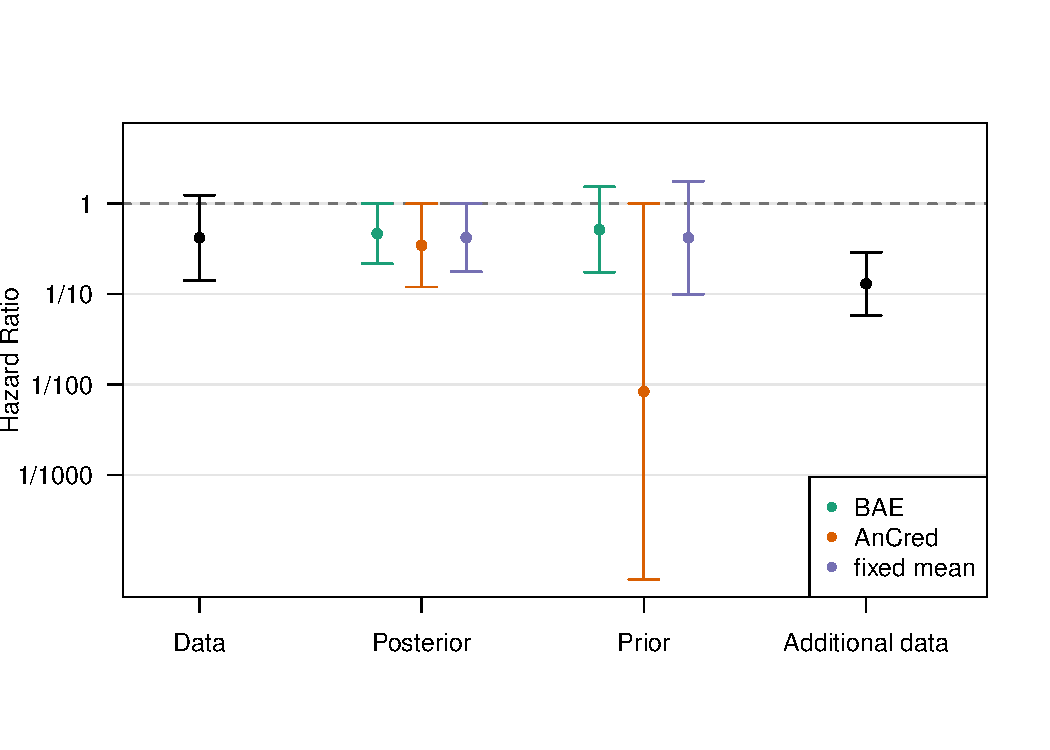
\includegraphics[width=\maxwidth]{images/paper5/bae-comparison-fig-1}
\end{knitrout}
\caption{Comparison of BAE, AnCred, and fixed mean 95\% prior and posterior
  credible intervals for the data from \citet{Sondhi2021}. Additional data from
  \citet{Innocenti2019} are also shown.}
\label{fig5:illustration}
\end{figure}


\begin{figure}[!htb]
\begin{knitrout}
\definecolor{shadecolor}{rgb}{0.969, 0.969, 0.969}\color{fgcolor}
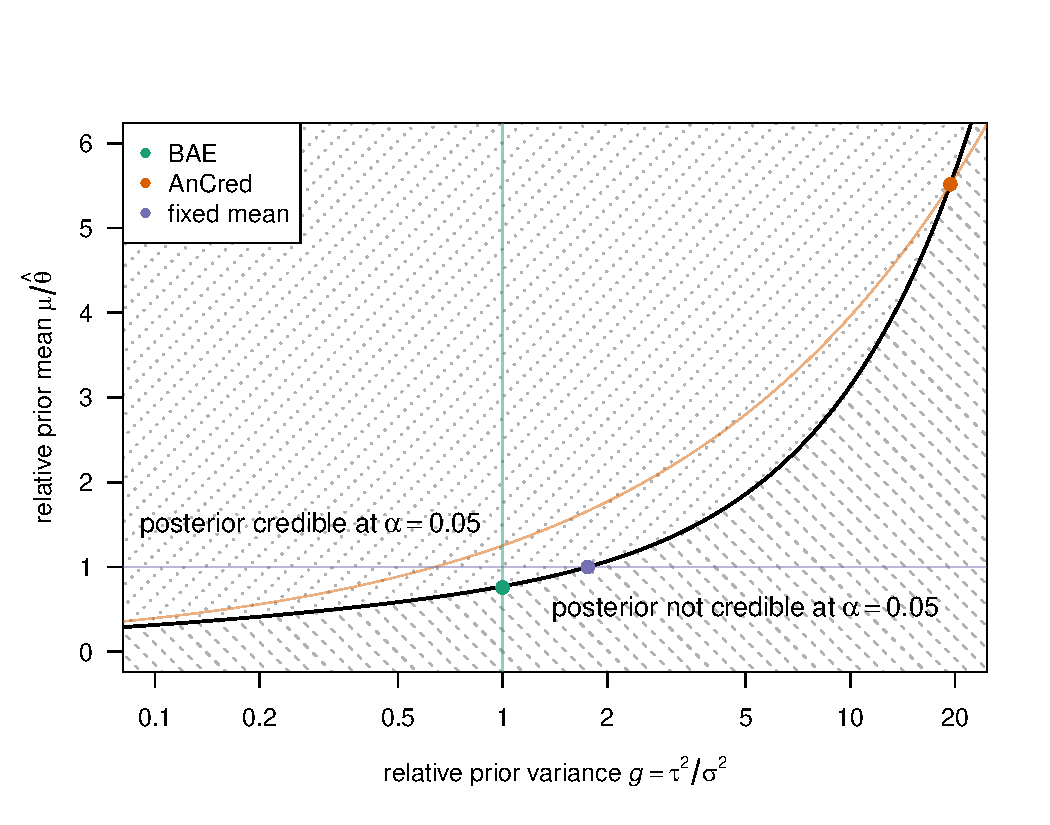
\includegraphics[width=\maxwidth]{images/paper5/plot-2d-1}
\end{knitrout}
\caption{Relative prior mean vs. relative prior variance for the data from
  Sondhi et al. The dashed region represents parameter values, which do not lead
  to posterior credibility, whereas values in the dotted region lead to
  posterior credibility (at $\alpha = 5\%$). The
  colored lines indicate the parameters which fulfil the side-constraints of the
  respective method.}
\label{fig5:priospace}
\end{figure}

\section{Alternatives approaches}
In order to get a unique solution for the BAE, Sondhi et al. make the assumption
that the prior variance equals the data variance, but also other possibilities
exist. An alternative rationale would be to set the mean of the additional
evidence, rather than variance, to that of the original finding (\ie{}
$\mu = \hat{\theta}$), and determining the prior variance $\tau^{2}$ such that
the posterior credible interval includes the null value. Under this approach,
the prior variance is given by
\begin{align*}
  \tau^{2} = \frac{\sigma^{2}}{z_{\scriptscriptstyle \alpha/2}^2/z^2 - 1}
\end{align*}
with $z = \hat{\theta}/\sigma$. The resulting prior represents a study with
identical effect estimate but different precision compared to the observed one.
As the observed study becomes more convincing (with larger effect estimates
$|\hat{\theta}|$ and/or smaller standard errors $\sigma$), the prior will become
more diffuse, so less additional evidence is needed to render the finding
credible. We see in Figure~\ref{fig5:illustration} that prior and posterior are
similar to BAE for the clinical trial data from Sondhi et al.


Figure~\ref{fig5:illustration} also illustrates that the BAE and the fixed mean
approach can lead to priors which support effect sizes opposing that of the
original finding. This is not possible with the AnCred advocacy prior whose
prior credible interval is fixed to the null value so that the prior adheres to
the Principle of Fairminded Advocacy \citep{Matthews2018}. \citet{Held2021b}
showed that this constraint is equivalent to fixing the coefficient of variation
from the prior to $\tau/\mu = z_{\scriptscriptstyle \alpha/2}^{-1}$. Hence, its
mean and variance are given by
\begin{align*}
  &\mu = \frac{2 \, \hat{\theta}}{1 - z^{2}/z_{\scriptscriptstyle \alpha/2}^{2}}&
  &\text{and}&
  &\tau^{2} = \frac{\mu^{2}}{z_{\scriptscriptstyle \alpha/2}^{2}}.&
\end{align*}
We see that -- as with the fixed mean approach -- the AnCred prior becomes more
diffuse for increasingly convincing studies. However, at the same time the prior
mean also increases (decreases) for positive (negative) effect estimates, so
that only effect sizes in the correct direction are supported.

Figure~\ref{fig5:illustration} shows that the AnCred advocacy prior credible
interval is far wider compared to the other approaches. Perhaps this observation
led Sondhi et al. to state that AnCred is harder to interpret than BAE, and that
it can lead to prior intervals ``wide enough to effectively contain any effect
size, which is unhelpful for decision making''. We would argue that broad priors
are a valuable diagnostic of when little additional evidence is needed to
achieve posterior credibility, as it is the case with the example Sondhi et al.
consider. Moreover, we would argue that AnCred priors are very helpful in
decision making since any additional evidence whose confidence interval is
contained in the AnCred prior credible interval will \emph{necessarily} lead to
posterior credibility when combined with the observed data \citep{Held2021b}. In
contrast, the BAE approach requires decision makers to keep in mind the variance
of the additional evidence, since only additional evidence with a point estimate
that is more extreme as the BAE and with confidence interval at least as tight
as the observed confidence interval from the study is guaranteed to lead to
posterior credibility. Assume, for example, the additional data from Innocenti
et al. had been more impressive, say, $\mbox{HR} = 0.05$, with a 95\% CI from
0.015 to 0.16. Intuition suggests, and direct calculation confirms, that this
would be even more capable of making the original finding credible. However,
this would not be clear to a decision maker using the BAE approach as currently
formulated, as the confidence interval is wider than the one of the observed
study (on the log scale).

While Sondhi et al. acknowledge the dependence of the BAE on the choice of the
prior variance, they do not give clear guidance on when it should be set to a
value different from the observed data variance. Fortunately, when the prior and
data variances differ, there is again a closed form solution for the BAE
``tipping point''
\begin{align}
  \text{BAE}(g)
  & =  \sign(\hat{\theta}) \sqrt{g \, (1 + g)} \, z_{\scriptscriptstyle \alpha/2} \, \sigma
    - g \, \hat{\theta}
    \label{eq5:bae2}
\end{align}
with relative prior variance $g = \tau^{2}/\sigma^{2}$. We see from
Figure~\ref{fig5:priospace} that Eq.~\eqref{eq5:bae2} substantially depends on the
chosen prior variance and that the BAE based on $g = 1$ only captures a limited
range of priors which lead to posterior credibility. Unfortunately, Sondhi et
al. do not give a clear rationale for the default choice of $g = 1$. It may
therefore be more helpful for decision makers to base their decision on the more
principled AnCred advocacy prior or on a visualisation of the prior parameter
space as in Figure~\ref{fig5:priospace}.

\section{Conclusion}
In summary, we welcome BAE as an interesting application of reverse-Bayes
methods, and we hope our derivation of closed-form solutions will encourage
further research. However, as currently formulated BAE lacks both a clear
rationale for the constraints on which it is based, and a sufficiently detailed
explanation allowing reliable decision-making.

\section*{Software and data}
Summary statistics on the case study were taken from \citet{Sondhi2021}. The
code to reproduce our analyses is available at
\url{https://github.com/SamCH93/BAEcomment}. A snapshot of the Git repository at
the time of writing is archived at \url{https://doi.org/10.5281/zenodo.7437722}.

\section*{Acknowledgments}
We thank two anonymous referees and the third referee Riko Kelter for their
helpful suggestions.%  Financial support from the Swiss National Science
% Foundation (Project \#189295) is gratefully acknowledged. The funder had no role
% in study design, data collection, data analysis, data interpretation, decision
% to publish, or preparation of the manuscript.

\bibliographystyle{apalikedoiurl}
\bibliography{bibliography}
